\documentclass{article}

\usepackage{summary}

\subject{Urheberrecht in der Informationsgesellschaft}
\semester{Summer 2024}
\author{Leopold Lemmermann}

\begin{document}\createtitle

\section{Geistiges Eigentum}
\begin{quote}
  Zeitlich beschränkter Schutz immateriellen, geistigen Inhalts. In Abgrenzung zu Sachenrechten, die sich auf materielle Gegenstände beziehen und zeitlich unbeschränkt sind.
\end{quote}

\begin{itemize}
  \item Ideelles Persönlichkeitsrecht: nicht veräußerlich \& zeitlich begrenzt
  \item Materielle, wirtschaftliche Rechte: Ansprüche.
\end{itemize}

Territorialität: Keine einheitliche Rechtsordnung, sondern nationale Gesetze.

Rechtsgrundsätze: lex-specialis, lex-posterior, lex-superior

\subsection{Normenpyramide im Urheberrecht}

Internationale Verträge: Universal Copyright Convention, TRIPS, WIPO Copyright Treaty, Berner Übereinkunft\\
Europarecht: diverse Richtlinien\\
Nationale Gesetze: UrhG, VGG, VerlG

\subsection{Kritik an EU-Reform von 2019}
Artikel 15 (Leistungsschutzrecht): Lizenzierungspflicht für Texte führt evtl. zu weniger Medienvielfalt.\\
Artikel 17 (Uploadfilter): Plattformbetreiber müssen Inhalte präventiv filtern, was zu Overblocking führen kann.

\subsection{Urheberrechts-Dienstanbieter-Gesetz (UrhDaG)}
Kritik an EU-Reform verarbeiten.
Lösungansatz
\begin{itemize}
  \item Blockierung nicht-lizenzierter Uploads: grds. erlaubte Nutzung annehmen (gg. Overblocking), per Red Button sofortiges Blockieren durch Rechteinhaber
  \item Meinungs- \& Kommunikationsfreiheit durhc präzisierte Schranken.
\end{itemize}
Ausnahmen für geringfügige Nutzung oder Satire, Parodie, etc…

\begin{figure}
  \resizebox{\textwidth}{!}{
    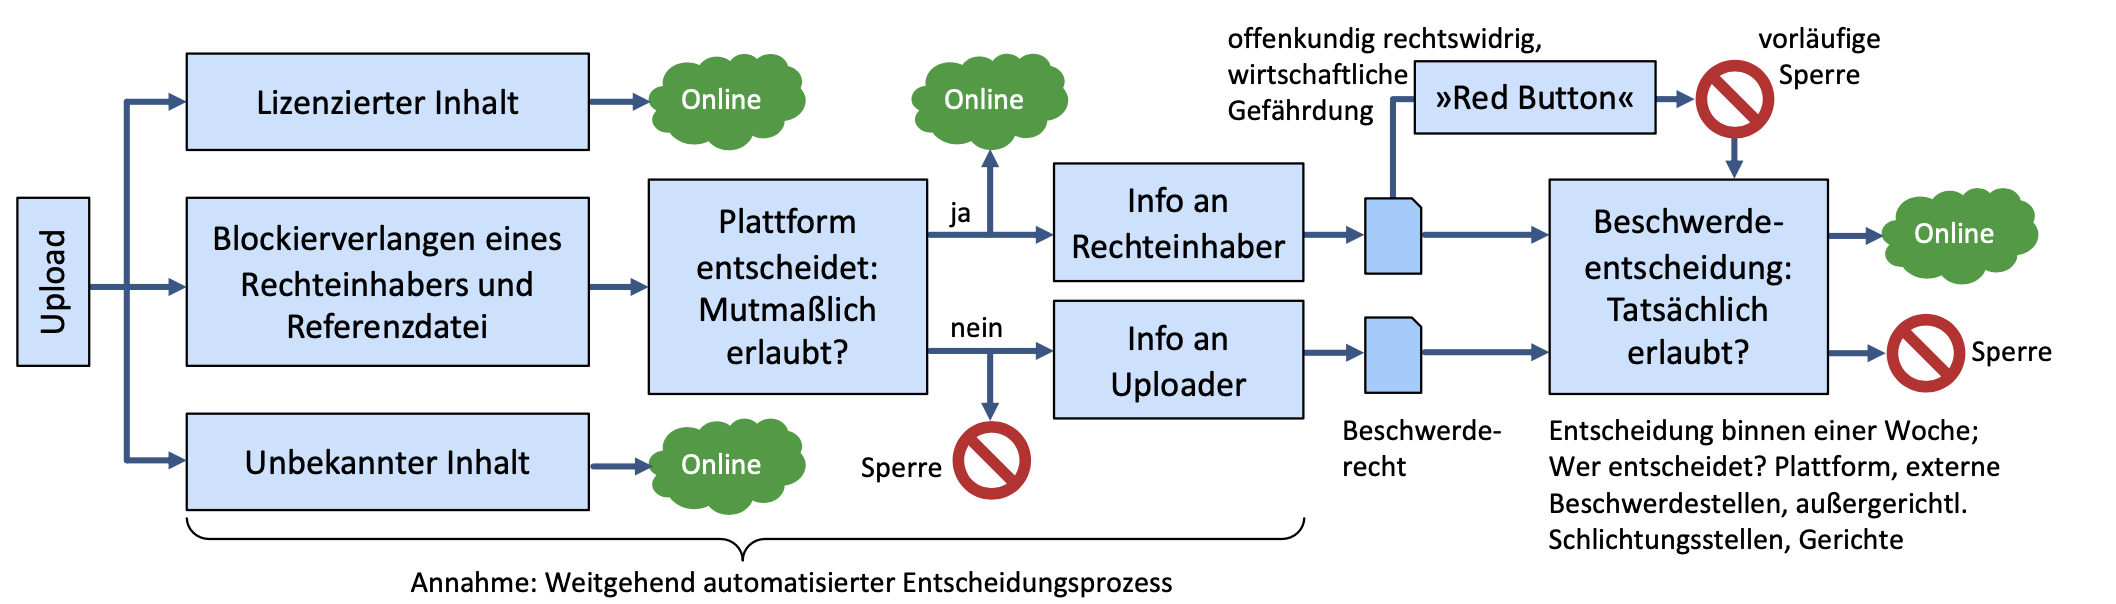
\includegraphics{res/uploads.png}
  }
  \caption{Uploads}
\end{figure}

\section{Urheberrechtsgesetz (UrhG)}
\begin{table}
  \centering
  \begin{tabular}{c|c|c|c|c}
    §§1-69       & §§70-87h           & §§88-95 & §§96-119              & §§120-143            \\
    Urheberrecht & verw. Schutzrechte & Filme   & geteilte Bestimmungen & Anwendungsbereich, …
  \end{tabular}
\end{table}

\end{document}